\documentclass{scrreprt}

\usepackage{aligned-overset}
\usepackage{amsmath}
\usepackage{amsthm}
\usepackage{amssymb}
\usepackage{bm}
\usepackage[shortlabels]{enumitem}
\usepackage{framed}
\usepackage{hyperref}
\usepackage[utf8]{inputenc}
\usepackage{multicol}
\usepackage{mathtools}
\usepackage{pdflscape}
\usepackage{physics}
\usepackage{polynom}
\usepackage{tabularx}
\usepackage[table]{xcolor}
\usepackage{titling}
\usepackage{fancyhdr}
\usepackage{xfrac}
\usepackage{pgfplots}

\pgfplotsset{compat = newest}
\usepgfplotslibrary{fillbetween}
\usetikzlibrary{calc}
\usetikzlibrary{patterns}
\usetikzlibrary{through}


\author{Karsten Lehmann \\ 4935758}
\date{WiSe 2024/25}
\title{Nachbereitungsaufgaben 12\\INF-B-110, Lineare Algebra}

\setlength{\headheight}{26pt}
\pagestyle{fancy}
\fancyhf{}
\lhead{\thetitle}
\rhead{\theauthor}
\lfoot{\thedate}
\rfoot{Seite \thepage}

\begin{document}
\paragraph{N 12.2} Es seien
$m_1 \quad m_2 \quad m_3 \quad m_4 \quad m_5 \quad m_6 \quad m_7$ die Ziffern
Ihrer Matrikelnummer.

Es sei $V$ der $\mathbb{R}$-Vektorraum $\mathbb{R}^4$ und
$s \colon V \times V \to \mathbb{R}$ das Standardskalarprodukt in $V$.
Weiter seien $v_1 = \qty\big(1, m_2, m_3, m_4)^T$ und
$v_2 = \qty\big(0, 1, m_6, m_7)^T$ Elemente von $V$ und
$U \coloneqq \text{Span}\qty\big{v_1, v_2}$.
\begin{enumerate}[(a)]
\item Berechnen Sie $2v_1 \bullet \frac{1}{2}v_2$.

  \subparagraph{Lsg.} Die einzelnen Ziffern der Matrikelnummer sind

  \begin{tabular}{|c|c|c|c|c|c|c|}
    \hline
    4 & 9 & 3 & 5 & 7 & 5 & 8 \\
    \hline
    $m_1$ & $m_2$ & $m_3$ & $m_4$ & $m_5$ & $m_6$ & $m_7$ \\
    \hline
  \end{tabular}

  und somit
  \[
    v_1 = \qty\big(1, 9, 3, 5)^T \text{ und }
    v_2 = \qty\big(0, 1, 5, 8)^T
  \]

  Nun ist
  \[
    2v_1 \bullet \frac{1}{2}v_2
    = 2\begin{pmatrix}
      1 \\
      9 \\
      3 \\
      5 \\
    \end{pmatrix} \bullet \frac{1}{2} \begin{pmatrix}
      0 \\
      1 \\
      5 \\
      8 \\
    \end{pmatrix}
    = \begin{pmatrix}
      2  \\
      18 \\
      6  \\
      10 \\
    \end{pmatrix} \bullet \begin{pmatrix}
      0           \\
      \frac{1}{2} \\
      \frac{5}{2} \\
      4           \\
    \end{pmatrix}
    = 2 \cdot 0 + 18 \cdot \frac{1}{2} + 6 \cdot \frac{5}{2} + 10 \cdot 4
    = 64
  \]
\item Finden Sie alle Vektoren $w \in \mathbb{R}^4$ , die den gleichen
  Abstand zu $v_1$ wie $v_2$ haben, für die also
  $\norm{v_1 - w} = \norm{v_2 - w}$ gilt.

  \subparagraph{Lsg.} Vorbetrachtung im $\mathbb{R}^2$ mit zwei Vektoren
  $v, w \in \mathbb{R}^2$:

  \begin{tikzpicture}
    \begin{axis}[
      axis equal image,
      axis x line=center,
      axis y line=center,
      grid=both,
      xmin=-0.5,
      xmax=2.5,
      xtick distance=1,
      xticklabel={\empty},
      ymin=-0.5,
      ymax=1.5,
      ytick distance=1,
      yticklabel={\empty},
    ]
    \node[circle, draw, inner sep=0pt, minimum size=1mm,label=above right:{$w$}] (w) at (1,1) {};
    \node[circle, draw, inner sep=0pt, minimum size=1mm,label=below right:{$v$}] (v) at (1,0.4) {};
    \node[circle, draw, inner sep=0pt, minimum size=1mm,label=above right:{$u'$}] (u) at (1,0.7) {};

    \node[circle, draw, inner sep=0pt, minimum size=1mm,label=above right:{$s_1$}] (s1) at (0.5,0.7) {};
    \node[circle, draw, inner sep=0pt, minimum size=1mm,label=above right:{$s_2$}] (s2) at (0.75,0.7) {};
    \node[circle, draw, inner sep=0pt, minimum size=1mm,label=above right:{$s_3$}] (s3) at (1.5,0.7) {};

    \draw[dotted] (s1) -- (w);
    \draw[dotted] (s1) -- (v);
    \draw[dotted] (s2) -- (w);
    \draw[dotted] (s2) -- (v);
    \draw[dotted] (s3) -- (w);
    \draw[dotted] (s3) -- (v);

    \draw[dashed, ->] (0, 0) -- (u);
    \draw[black!10!blue, line width=0.25mm] (-0.5, 0.7) -- (2.5, 0.7);
    \end{axis}
  \end{tikzpicture}

  Punkte $s_1, s_2, s_3$ mit gleichem Abstand zu $v$ und $w$ liegen auf einer
  Hyperebene, die Senkrecht zu $w - v$ ist und durch den Mittelpunkt
  $u' = v + \frac{w - v}{2}$ zwischen $v$ und $w$ verläuft.

  Sei nun
  $X = \text{Span}\qty\big{v_2 - v_1}
  = \text{Span}\qty{\qty\big(-1, -8, 2, 3)^T}$.
  Dann ist
  \begin{flalign*}
    X^{\bot} = \text{Ker}\qty\big(u)
    &= \text{Ker}\begin{pmatrix}
      -1 & -8 & 2 & 3 \\
    \end{pmatrix} \\
    &= \text{Ker}\begin{pmatrix}
      1 & 8 & -2 & -3 \\
    \end{pmatrix} \\
    &= \qty{
      \begin{pmatrix}
        -8b + 2c + 3d \\
        b             \\
        c             \\
        d             \\
      \end{pmatrix}
      \:\middle|\:
      b, c, d \in \mathbb{R}
    } \\
    &= \qty{
      b \cdot \begin{pmatrix}
        -8 \\
        1  \\
        0  \\
        0  \\
      \end{pmatrix} + c \cdot \begin{pmatrix}
        2 \\
        0 \\
        1 \\
        0 \\
      \end{pmatrix} + d \cdot \begin{pmatrix}
        3 \\
        0 \\
        0 \\
        1 \\
      \end{pmatrix}
      \:\middle|\:
      b, c, d \in \mathbb{R}
    } \\
    &= \text{Span}\qty{
      \begin{pmatrix}
        -8 \\
        1  \\
        0  \\
        0  \\
      \end{pmatrix}, \begin{pmatrix}
        2 \\
        0 \\
        1 \\
        0 \\
      \end{pmatrix}, \begin{pmatrix}
        3 \\
        0 \\
        0 \\
        1 \\
      \end{pmatrix}
    }
  \end{flalign*}

  Nun verläuft $X^{\bot}$ bereits orthogonal zu $v_2 - v_1$,
  allerdings verläuft $X^{\bot}$ noch nicht durch den Mittelpunkt
  $u = v_1 + \frac{v_2 - v_1}{2} = \qty\big(\frac{1}{2}, 5, 4, \frac{13}{2})^T$
  von $v_1$ und $v_2$.

  Die Lösungsmenge ist die Hyperebene, welche durch eine Verschiebung vom
  Orthogonalraum $X^{\bot}$ um $u$ entsteht:
  \[
    L = X^{\bot} + u
    = \qty{
      b \cdot \begin{pmatrix}
        -8 \\
        1  \\
        0  \\
        0  \\
      \end{pmatrix} + c \cdot \begin{pmatrix}
        2 \\
        0 \\
        1 \\
        0 \\
      \end{pmatrix} + d \cdot \begin{pmatrix}
        3 \\
        0 \\
        0 \\
        1 \\
      \end{pmatrix} + \begin{pmatrix}
        \frac{1}{2} \\
        5           \\
        4           \\
        \frac{13}{2} \\
      \end{pmatrix}
      \:\middle|\:
      b, c, d \in \mathbb{R}
    }
  \]

  \textbf{Probe:} Sei
  \[
    s = \qty(
      1 \cdot \begin{pmatrix}
        -8 \\
        1  \\
        0  \\
        0  \\
      \end{pmatrix} + 2 \cdot \begin{pmatrix}
        2 \\
        0 \\
        1 \\
        0 \\
      \end{pmatrix} + 3 \cdot \begin{pmatrix}
        3 \\
        0 \\
        0 \\
        1 \\
      \end{pmatrix} + \begin{pmatrix}
        \frac{1}{2} \\
        5           \\
        4           \\
        \frac{13}{2} \\
      \end{pmatrix}
      ) = \begin{pmatrix}
      \frac{11}{2} \\
      6            \\
      6            \\
      \frac{19}{2} \\
    \end{pmatrix}
  \]
  Dann ist
  \[
    \norm{v_1 - s} = \norm{\qty\big(-\frac{9}{2}, 3, -3, -\frac{9}{2})^T}
    = \sqrt{\frac{117}{2}}
    \text{ und }
    \norm{v_2 - s} = \norm{\qty\big(-\frac{11}{2}, -5, -1, -\frac{3}{2})^T}
    = \sqrt{\frac{117}{2}}
  \]

\item Bestimmen Sie die Dimension des Orthogonalraums $U^{\bot}$ von $U$.

  \subparagraph{Lsg.} Es gilt
  $\text{dim}\qty\big(V) - \text{dim}\qty\big(U) = \text{dim}\qty\big(U^{\bot})$.
  Nun ist $\text{dim}\qty\big(V) = 4$ und da $v_1$ und $v_2$ offensichtlich
  linear unabhängig sind (betrachte das erste Element von $v_1$ und $v_2$),
  ist $\text{dim}\qty\big(U) = 2$

  Somit ist auch $\text{dim}\qty\big(U^{\bot}) = 2$

\newpage
\item Berechnen Sie eine Basis des Orthogonalraums $U^{\bot}$ von $U$.

  \subparagraph{Lsg.} Ein Vektor $w = \qty\big(a, b, c, d)^T \in V$ ist in
  $U^{\bot}$, falls er zu $v_1$ und $v_2$ orthogonal ist, dass heißt
  \[
    1 \cdot a + 9 \cdot b + 3 \cdot c + 5 \cdot d = 0 =
    0 \cdot a + 1 \cdot b + 5 \cdot c + 8 \cdot d
  \]
  Somit ist der Orthogonalraum von $U$ gleich
  \begin{flalign*}
    \text{Ker}\begin{pmatrix}
      1 & 9 & 3 & 5 \\
      0 & 1 & 5 & 8 \\
    \end{pmatrix}
    \overset{Z_1 + Z_1 - 9 \cdot Z_2}&=
    \text{Ker}\begin{pmatrix}
      1 & 0 & -42 & -67 \\
      0 & 1 & 5   & 8   \\
    \end{pmatrix} \\
    &= \qty{
      \begin{pmatrix}
        42 \cdot c + 67 \cdot d \\
        -5 \cdot c - 8 \cdot d  \\
        c                       \\
        d                       \\
      \end{pmatrix}
      \:\middle|\:
      c, d \in \mathbb{R}
    } \\
    &= \qty{
      c \cdot \begin{pmatrix}
        42 \\
        -5 \\
        1  \\
        d  \\
      \end{pmatrix} + d \cdot \begin{pmatrix}
        67 \\
        -8 \\
        0  \\
        1  \\
      \end{pmatrix}
      \:\middle|\:
      c, d \in \mathbb{R}
    } \\
    &= \text{Span}\qty{
      \begin{pmatrix}
        42 \\
        -5 \\
        1  \\
        0  \\
      \end{pmatrix}, \begin{pmatrix}
        67 \\
        -8 \\
        0  \\
        1  \\
      \end{pmatrix}
    }
  \end{flalign*}
  und $\qty{\qty\big(42, -5, 1, 0)^T,\qty\big(67, -8, 0, 1)^T}$ eine Basis von
  $U^{\bot}$.
\newpage
\item Beweisen Sie:
  $\forall v, w \in V \colon \norm{v} = \norm{w}
  \Rightarrow \qty\big(v + w) \bot \qty\big(v - w)$

  \subparagraph{Lsg.}
  Es ist
  \begin{flalign*}
    \norm{w} &= \norm{v} && {\Big |} \qty\big(\ldots)^2 \\
    \norm{w}^2 &= \norm{v}^2 && {\Big |} - \norm{w}^2 \\
    0 &= \norm{v}^2 - \norm{w}^2 \\
    \overset{\text{Def. Norm}}&= \sqrt{v \bullet b}^2 - \sqrt{w \bullet w}^2 \\
    &= v \bullet v - w \bullet w \\
    &= v \bullet v + \qty\big(v \bullet w - v \bullet w) - w \bullet w \\
    \overset{\text{Symmetrisch}}&= v \bullet v + \qty\big(w \bullet v - v \bullet w) - w \bullet w \\
    &= v \bullet v + \qty\big(- v \bullet w + w \bullet v) - w \bullet w \\
    &= v \bullet v - v \bullet w + w \bullet v - w \bullet w \\
    \overset{\text{bilinear}}&= v \bullet \qty\big(v - w) + w \bullet \qty\big(v - w) \\
    0 \overset{\text{bilinear}}&= \qty\big(v + w) \bullet \qty\big(v - w)
  \end{flalign*}
  und somit sind $\qty\big(v + w)$ und $\qty\big(v - w)$ orthogonal zueinander,
  da ihr Skalarprodukt 0 ist.
\end{enumerate}
\end{document}
